%* 
%* ------------------------------------------------------------------
%* ApplicationNote02.tex - Application Note 02: Two Siding Oval N
%* Created by Robert Heller on Sun Sep 16 08:44:31 2012
%* ------------------------------------------------------------------
%* Modification History: $Log$
%* Modification History: Revision 1.1  2002/07/28 14:03:50  heller
%* Modification History: Add it copyright notice headers
%* Modification History:
%* ------------------------------------------------------------------
%* Contents:
%* ------------------------------------------------------------------
%*  
%*     Model RR System, Version 2
%*     Copyright (C) 1994,1995,2002-2012  Robert Heller D/B/A Deepwoods Software
%* 			51 Locke Hill Road
%* 			Wendell, MA 01379-9728
%* 
%*     This program is free software; you can redistribute it and/or modify
%*     it under the terms of the GNU General Public License as published by
%*     the Free Software Foundation; either version 2 of the License, or
%*     (at your option) any later version.
%* 
%*     This program is distributed in the hope that it will be useful,
%*     but WITHOUT ANY WARRANTY; without even the implied warranty of
%*     MERCHANTABILITY or FITNESS FOR A PARTICULAR PURPOSE.  See the
%*     GNU General Public License for more details.
%* 
%*     You should have received a copy of the GNU General Public License
%*     along with this program; if not, write to the Free Software
%*     Foundation, Inc., 675 Mass Ave, Cambridge, MA 02139, USA.
%* 
%*  
%* 

\documentclass[12pt,notitlepage,twoside]{book}
\usepackage{svninfo}
\svnInfo $Id$
\usepackage{graphicx}
\usepackage{mathptm}
\usepackage{times}
\usepackage{makeidx}
\usepackage{MyTitlepage}
\usepackage{MyBibIndex}
\usepackage{url}
\usepackage{listings}
\usepackage{subfigure}
\pagestyle{headings}
\makeindex
\emergencystretch=50pt
\setcounter{tocdepth}{3}
\setcounter{secnumdepth}{3}
\begin{document}
\lstset{language=Tcl,basicstyle=\footnotesize,numbers=left,stepnumber=5}% Most examples will be in Tcl
\typeout{$Id$}
\newcommand{\MRRSubTitle}{Application Note 02: Two Siding Oval N}
%* 
%* ------------------------------------------------------------------
%* titlepage.tex - Common documentation title page
%* Created by Robert Heller on Sun Oct 13 15:59:49 2002
%* ------------------------------------------------------------------
%* Modification History: $Log$
%* Modification History: Revision 1.3  2007/10/22 17:17:27  heller
%* Modification History: 10222007
%* Modification History:
%* Modification History: Revision 1.2  2004/04/14 23:20:24  heller
%* Modification History: Updated copyright.
%* Modification History:
%* Modification History: Revision 1.1  2002/10/17 00:02:24  heller
%* Modification History: Documentation support files.
%* Modification History:
%* Modification History: Revision 1.1  2002/07/28 14:03:50  heller
%* Modification History: Add it copyright notice headers
%* Modification History:
%* ------------------------------------------------------------------
%* Contents:
%* ------------------------------------------------------------------
%*  
%*     Model RR System, Version 2
%*     Copyright (C) 1994,1995,2002  Robert Heller D/B/A Deepwoods Software
%* 			51 Locke Hill Road
%* 			Wendell, MA 01379-9728
%* 
%*     This program is free software; you can redistribute it and/or modify
%*     it under the terms of the GNU General Public License as published by
%*     the Free Software Foundation; either version 2 of the License, or
%*     (at your option) any later version.
%* 
%*     This program is distributed in the hope that it will be useful,
%*     but WITHOUT ANY WARRANTY; without even the implied warranty of
%*     MERCHANTABILITY or FITNESS FOR A PARTICULAR PURPOSE.  See the
%*     GNU General Public License for more details.
%* 
%*     You should have received a copy of the GNU General Public License
%*     along with this program; if not, write to the Free Software
%*     Foundation, Inc., 675 Mass Ave, Cambridge, MA 02139, USA.
%* 
%*  
%* 
%* 
%* $Id$  
%* 

\title{Model Railroad System \\ A collection of utilities for Model Railroaders\\ \MRRSubTitle}
\author{Robert Heller \\ Deepwoods Software \\ Wendell, MA, USA}
\date{\today}
\begin{titlepage}

\maketitle

%\begin{centering}
%\epsfig{file=../Cover1.ps} \\
%\end{centering}

\clearpage


This documentation was prepared with \LaTeX.

This document describes version 2 of the Model Railroad System package.

\vspace{.25in}



{\small Copyright \copyright 1994,1995,2002-2012 by Robert Heller D/B/A Deepwoods
Software}

\vspace{.25in}

All rights reserved.  Permission is granted to copy this document in
electronic form only, so long as it is with the software it
documents. 

The author, Robert Heller, may be contacted electronically (E-Mail) via
the following:

\begin{description}
\item[FidoNet] 1:321/153, Locks Hill BBS.
\item[InterNet] heller@deepsoft.com
\end{description}

Web site URL: {\tt http://www.deepsoft.com/}.

\thispagestyle{empty}
\setcounter{page}{0}
\clearpage

\end{titlepage}


\pagenumbering{roman}
\tableofcontents
\lstlistoflistings
\listoffigures
\listoftables
\cleardoublepage
%       
\cleardoublepage
\pagenumbering{arabic}
%
%* 
%* ------------------------------------------------------------------
%* AN02_Introduction.tex - Application Note 02: Introduction
%* Created by Robert Heller on Thu Sep 20 08:34:53 2012
%* ------------------------------------------------------------------
%* Modification History: $Log$
%* Modification History: Revision 1.1  2002/07/28 14:03:50  heller
%* Modification History: Add it copyright notice headers
%* Modification History:
%* ------------------------------------------------------------------
%* Contents:
%* ------------------------------------------------------------------
%*  
%*     Model RR System, Version 2
%*     Copyright (C) 1994,1995,2002-2012  Robert Heller D/B/A Deepwoods Software
%* 			51 Locke Hill Road
%* 			Wendell, MA 01379-9728
%* 
%*     This program is free software; you can redistribute it and/or modify
%*     it under the terms of the GNU General Public License as published by
%*     the Free Software Foundation; either version 2 of the License, or
%*     (at your option) any later version.
%* 
%*     This program is distributed in the hope that it will be useful,
%*     but WITHOUT ANY WARRANTY; without even the implied warranty of
%*     MERCHANTABILITY or FITNESS FOR A PARTICULAR PURPOSE.  See the
%*     GNU General Public License for more details.
%* 
%*     You should have received a copy of the GNU General Public License
%*     along with this program; if not, write to the Free Software
%*     Foundation, Inc., 675 Mass Ave, Cambridge, MA 02139, USA.
%* 
%*  
%* 

\chapter{Introduction}
\label{chapt:Introduction}
\typeout{$Id$}

This application note presents the hardware and software for a 2' by 6'
N continious running oval layout.  This module is a table top module
and features a single track oval with a pair of passing sidings.  It is
set up to run two trains in \textit{opposite} directions and does so in
a fully automated way using computer control, using USB connected IR
sensors and control modules from Azatrax.


%* 
%* ------------------------------------------------------------------
%* AN02_TheLayout.tex - Application Note 02: The Layout
%* Created by Robert Heller on Thu Sep 20 08:40:38 2012
%* ------------------------------------------------------------------
%* Modification History: $Log$
%* Modification History: Revision 1.1  2002/07/28 14:03:50  heller
%* Modification History: Add it copyright notice headers
%* Modification History:
%* ------------------------------------------------------------------
%* Contents:
%* ------------------------------------------------------------------
%*  
%*     Model RR System, Version 2
%*     Copyright (C) 1994,1995,2002-2012  Robert Heller D/B/A Deepwoods Software
%* 			51 Locke Hill Road
%* 			Wendell, MA 01379-9728
%* 
%*     This program is free software; you can redistribute it and/or modify
%*     it under the terms of the GNU General Public License as published by
%*     the Free Software Foundation; either version 2 of the License, or
%*     (at your option) any later version.
%* 
%*     This program is distributed in the hope that it will be useful,
%*     but WITHOUT ANY WARRANTY; without even the implied warranty of
%*     MERCHANTABILITY or FITNESS FOR A PARTICULAR PURPOSE.  See the
%*     GNU General Public License for more details.
%* 
%*     You should have received a copy of the GNU General Public License
%*     along with this program; if not, write to the Free Software
%*     Foundation, Inc., 675 Mass Ave, Cambridge, MA 02139, USA.
%* 
%*  
%* 

\chapter{The Layout}
\label{chapt:TheLayout}
\typeout{$Id$}

\begin{figure}[hbpt]
\begin{centering}
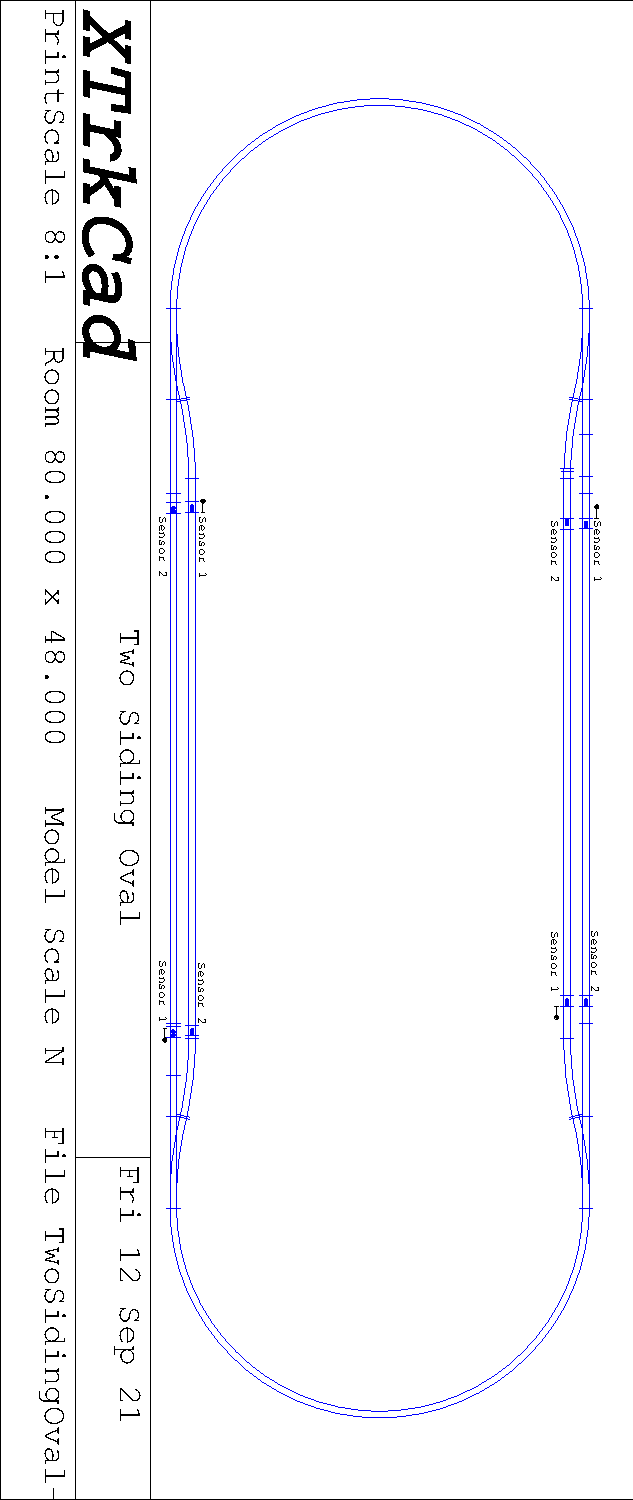
\includegraphics[angle=90,width=5in]{TwoSidingOval-N.pdf}
\caption{Two Siding Oval N}
\label{fig:TheLayout:TwoSidingOval-N}
\end{centering}
\end{figure}
The complete layout is shown in
Figure~\ref{fig:TheLayout:TwoSidingOval-N}. This is a basic oval with a
pair of passing sidings, one on each straight section. The turnouts at
the ends of the passing sidings will be controled by the computer to
allow continious running of two trains going in \textit{opposite}
directions.  If necessary, a train will be held at the end of its
siding until the other train clears the single track segment. The
computer will use Azatrax MRD2-U IR sensors to sense when the single
track segments are occupied and will use Azatrax SR4-U modules to
control the  direction of travel on the single track segments as well
as energizing the twin-coil switch machines to throw the turnouts as
needed. The trains will be plain DC powered and the rails will have gaps
to isolate the various power sections.  The single track segments will
be power from computer controlled reversing relays since these segments
will be operating in alternating directions.  The sidings will be fixed
polarity wired.

\begin{figure}[hbpt]
\begin{centering}
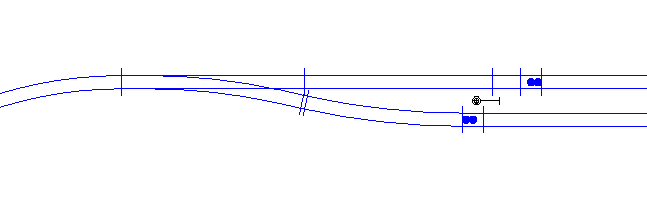
\includegraphics{TwoSidingOval-N-NW-Switch-sig-sensor.png}
\caption{Two Siding Oval N, North West Switch with Signal and Sensor locations}
\label{fig:TheLayout:TwoSidingOval-N-NW-Switch-sig-sensor}
\end{centering}
\end{figure}
Figure~\ref{fig:TheLayout:TwoSidingOval-N-NW-Switch-sig-sensor} shows
the detail of the North West Switch with the signal and sensor
locations. This is typical for each corner. The inner siding is counter
clockwise running and the outer siding is clockwise
running\footnote{This happens to correspond to ``lefthand'' running.}.  


%%* 
%* ------------------------------------------------------------------
%* AN02_Turnouts.tex - Application Note 02: Turnout Controls
%* Created by Robert Heller on Thu Sep 20 12:47:41 2012
%* ------------------------------------------------------------------
%* Modification History: $Log$
%* Modification History: Revision 1.1  2002/07/28 14:03:50  heller
%* Modification History: Add it copyright notice headers
%* Modification History:
%* ------------------------------------------------------------------
%* Contents:
%* ------------------------------------------------------------------
%*  
%*     Model RR System, Version 2
%*     Copyright (C) 1994,1995,2002-2012  Robert Heller D/B/A Deepwoods Software
%* 			51 Locke Hill Road
%* 			Wendell, MA 01379-9728
%* 
%*     This program is free software; you can redistribute it and/or modify
%*     it under the terms of the GNU General Public License as published by
%*     the Free Software Foundation; either version 2 of the License, or
%*     (at your option) any later version.
%* 
%*     This program is distributed in the hope that it will be useful,
%*     but WITHOUT ANY WARRANTY; without even the implied warranty of
%*     MERCHANTABILITY or FITNESS FOR A PARTICULAR PURPOSE.  See the
%*     GNU General Public License for more details.
%* 
%*     You should have received a copy of the GNU General Public License
%*     along with this program; if not, write to the Free Software
%*     Foundation, Inc., 675 Mass Ave, Cambridge, MA 02139, USA.
%* 
%*  
%* 

\chapter{Turnout Controls}
\label{chapt:Turnouts}
\typeout{$Id$}

\begin{figure}[hbpt]
\begin{centering}
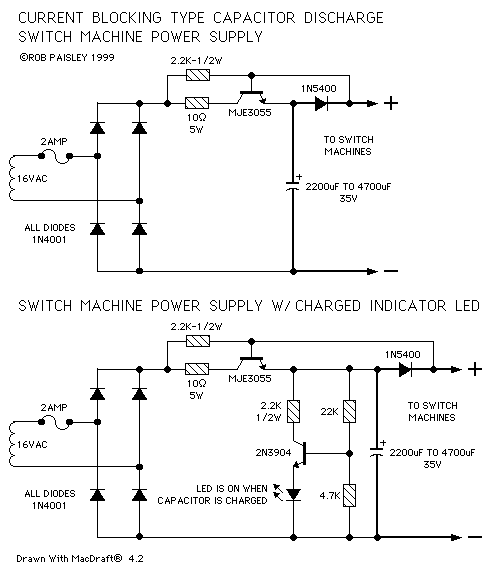
\includegraphics[width=5in]{CDblock.png}
\caption{Current Blocking Type Capacitor Discharge Switch Machine Power Supply}
\label{fig:Turnouts:CDblock}
\end{centering}
\end{figure}
\begin{figure}[hbpt]
\begin{centering}
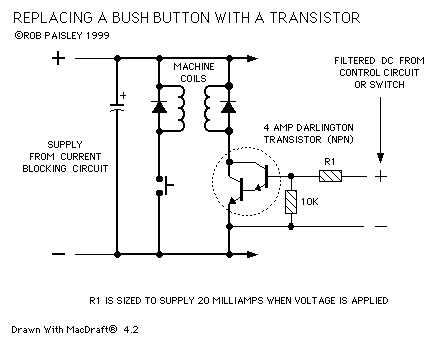
\includegraphics[width=5in]{CDtransistor.png}
\caption{Transisor control circuit}
\label{fig:Turnouts:CDtransistor}
\end{centering}
\end{figure}
\begin{figure}[hbpt]
\begin{centering}
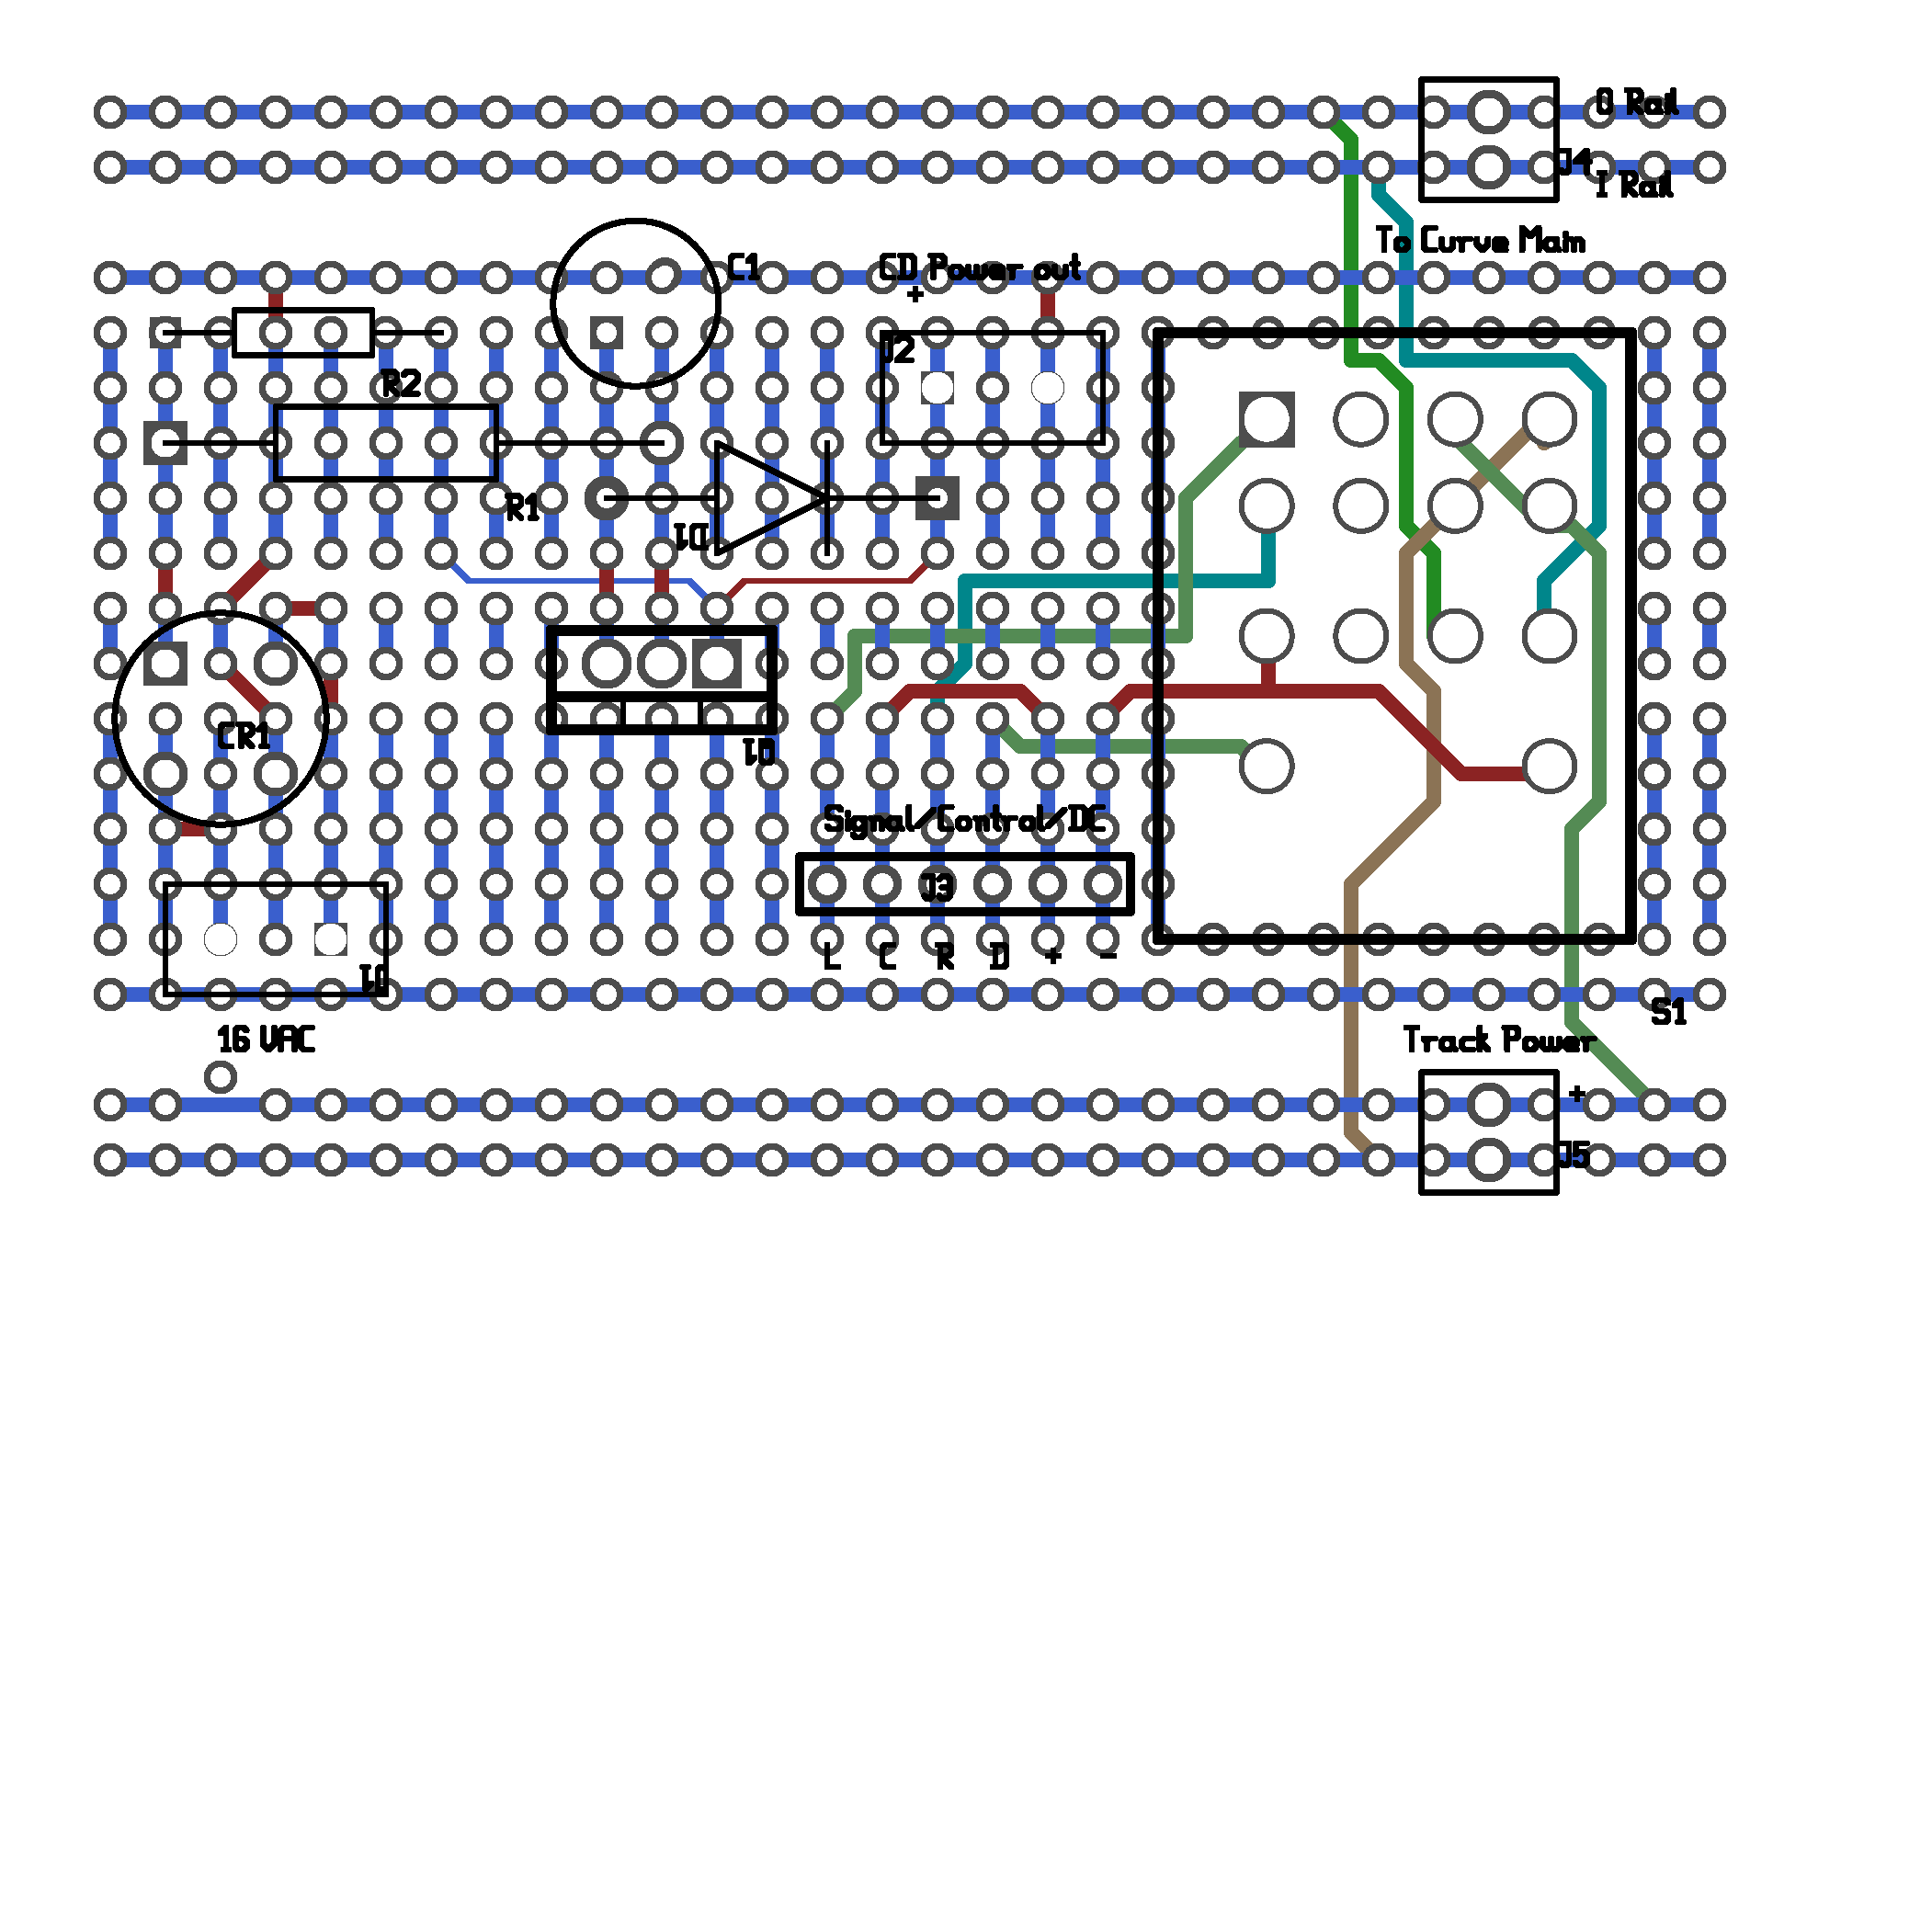
\includegraphics[width=5in]{CD-on-SB400.pdf}
\caption{Capacitor Discharge Power Supply Circuit Board}
\label{fig:Turnouts:CD-on-SB400}
\end{centering}
\end{figure}
\begin{figure}[hbpt]
\begin{centering}
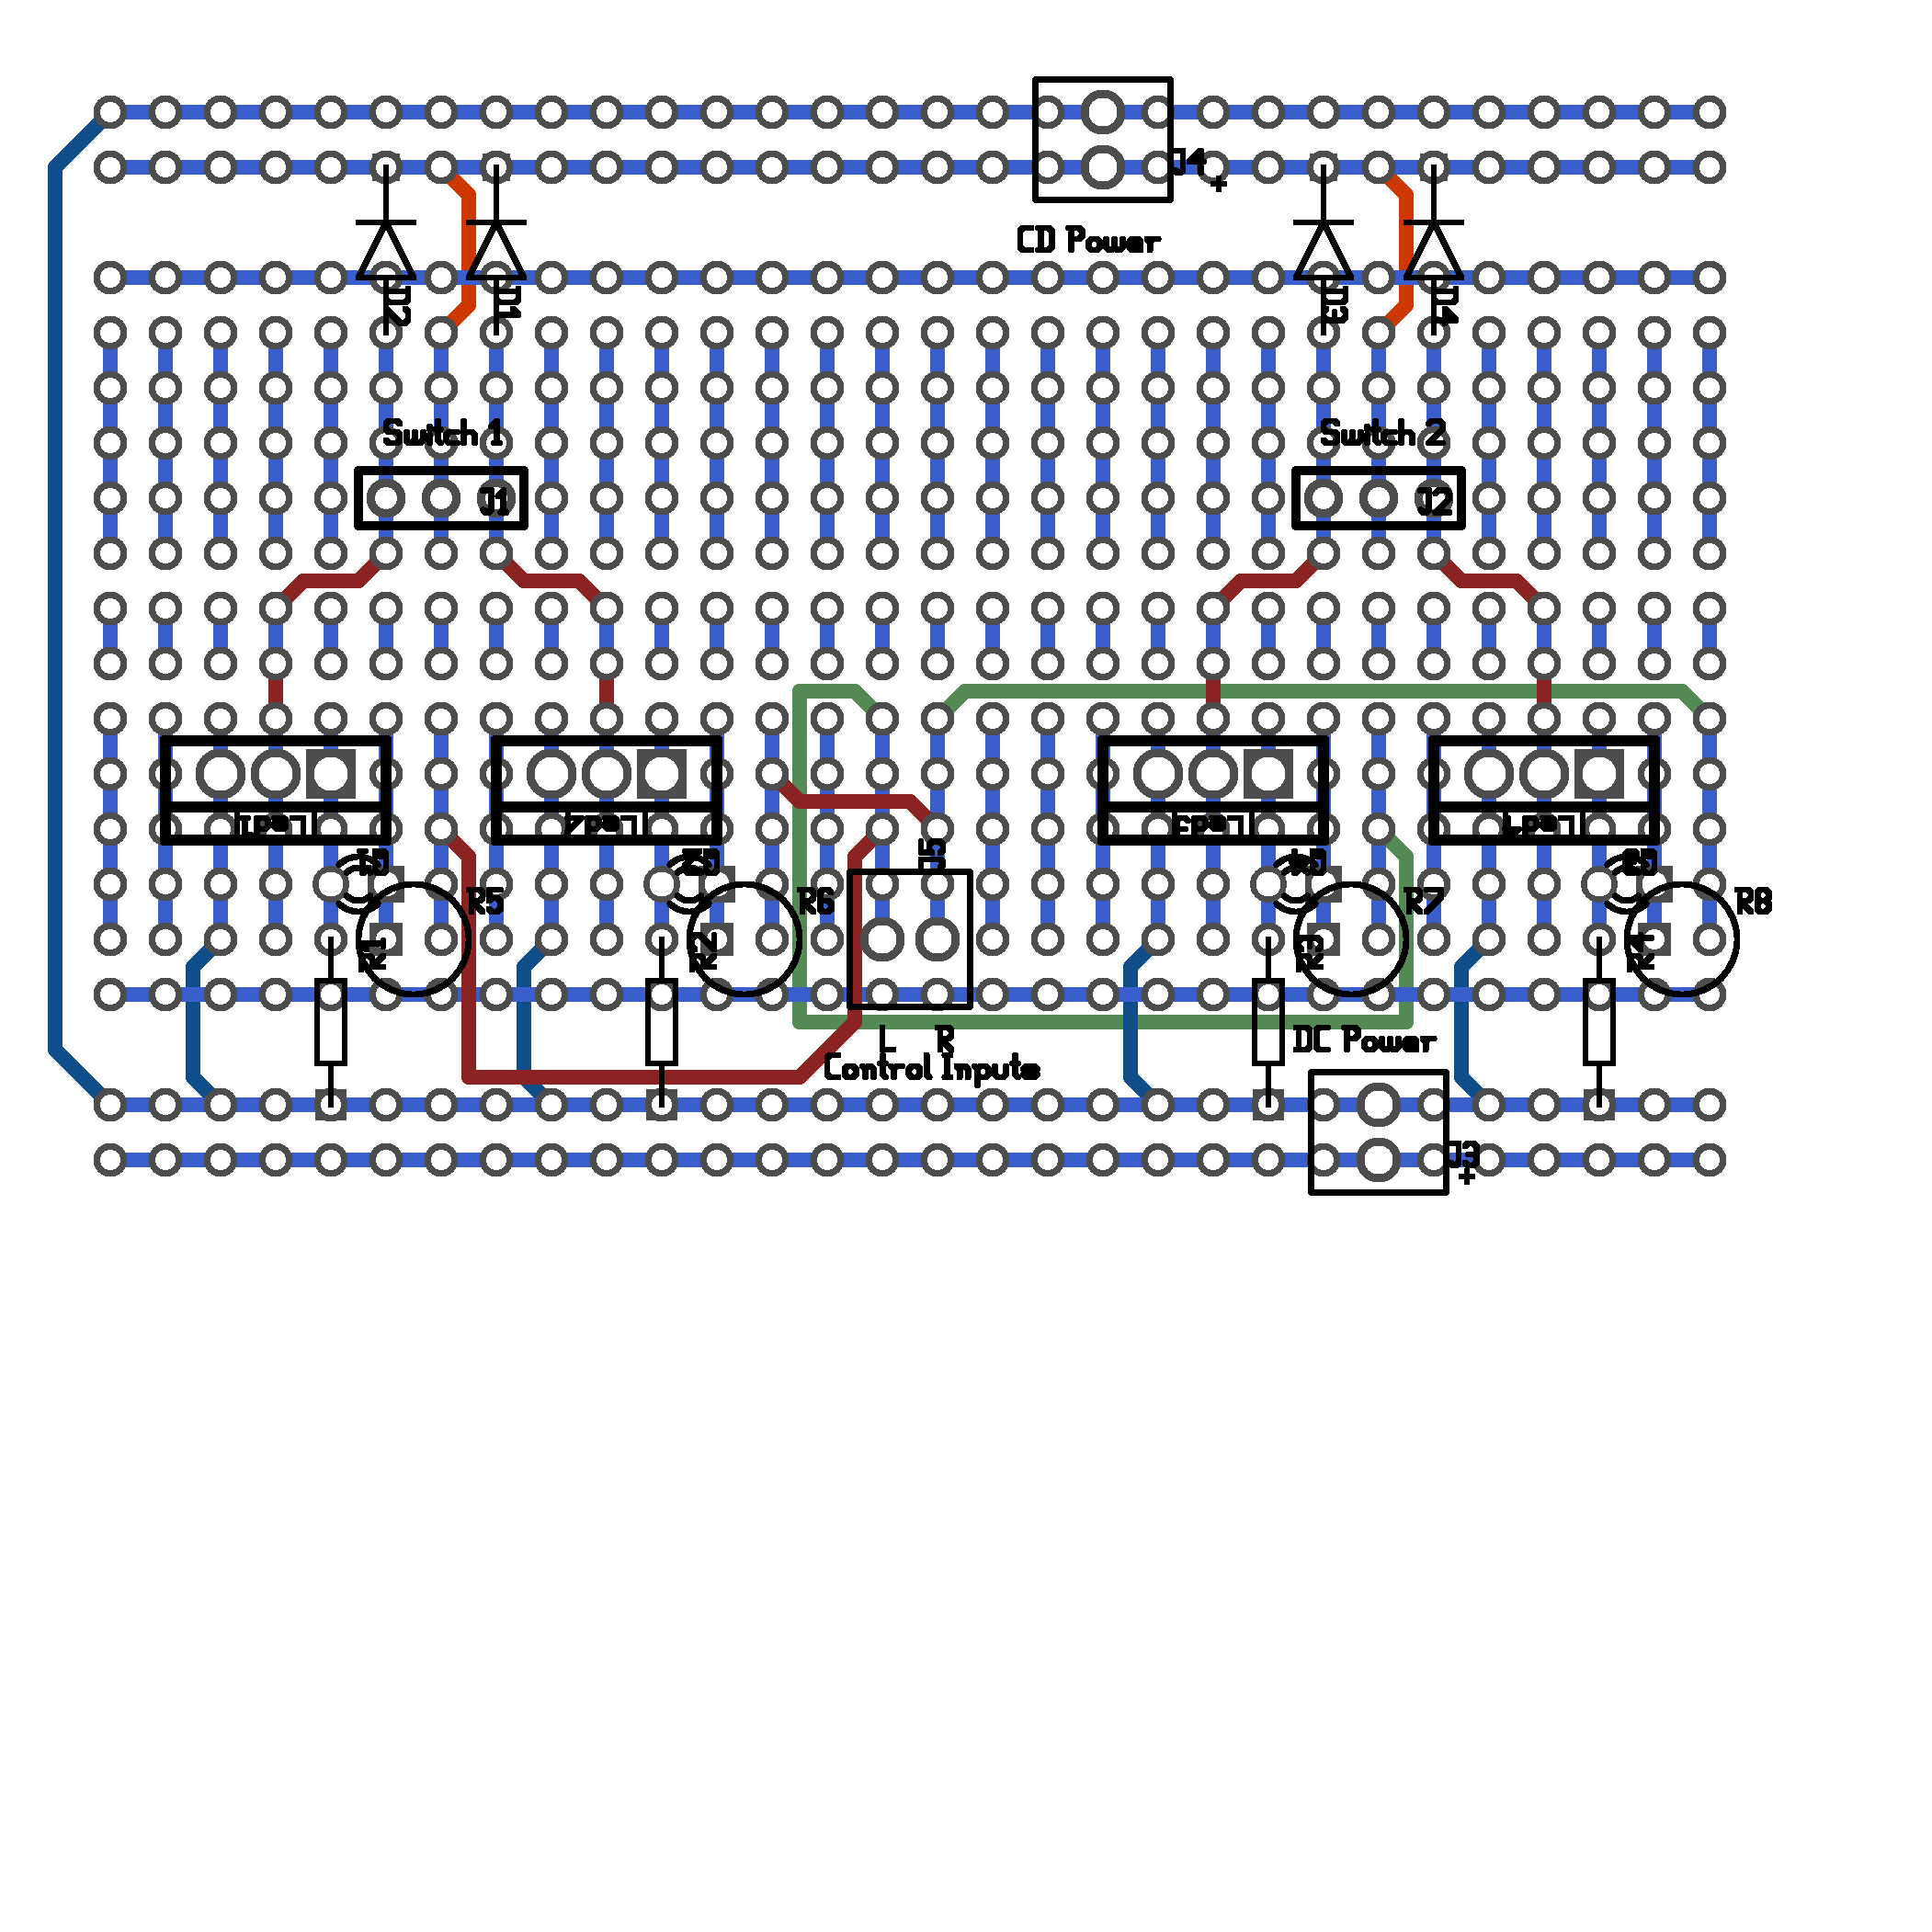
\includegraphics[width=5in]{4-CDtransistor-on-SB400.pdf}
\caption{4 transistor Switch Machine control Circuit Board}
\label{fig:Turnouts:4-CDtransistor-on-SB400}
\end{centering}
\end{figure}
The turnouts on this are controlled by twin-coil switch machines
mounted under the switches\footnote{Peco twin-coil switch machines.}.
We will be using current blocking type capacitor discharge switch
machine power supplies (Figure~\ref{fig:Turnouts:CDblock}), one for
each end of the layout, with power Darlington transistor control
circuits (Figure~\ref{fig:Turnouts:CDtransistor}).  We will build these
circuits on solderable breadboards, using circuit layouts shown in
Figures~\ref{fig:Turnouts:CD-on-SB400}\footnote{The power relay circuit
is also on this circuit board.} and \ref{fig:Turnouts:4-CDtransistor-on-SB400}. 


%%* 
%* ------------------------------------------------------------------
%* AN02_PowerRelay.tex - Application Note 02: Track Power Relay Circuit
%* Created by Robert Heller on Thu Sep 20 12:42:40 2012
%* ------------------------------------------------------------------
%* Modification History: $Log$
%* Modification History: Revision 1.1  2002/07/28 14:03:50  heller
%* Modification History: Add it copyright notice headers
%* Modification History:
%* ------------------------------------------------------------------
%* Contents:
%* ------------------------------------------------------------------
%*  
%*     Model RR System, Version 2
%*     Copyright (C) 1994,1995,2002-2012  Robert Heller D/B/A Deepwoods Software
%* 			51 Locke Hill Road
%* 			Wendell, MA 01379-9728
%* 
%*     This program is free software; you can redistribute it and/or modify
%*     it under the terms of the GNU General Public License as published by
%*     the Free Software Foundation; either version 2 of the License, or
%*     (at your option) any later version.
%* 
%*     This program is distributed in the hope that it will be useful,
%*     but WITHOUT ANY WARRANTY; without even the implied warranty of
%*     MERCHANTABILITY or FITNESS FOR A PARTICULAR PURPOSE.  See the
%*     GNU General Public License for more details.
%* 
%*     You should have received a copy of the GNU General Public License
%*     along with this program; if not, write to the Free Software
%*     Foundation, Inc., 675 Mass Ave, Cambridge, MA 02139, USA.
%* 
%*  
%* 


\chapter{Track Power Relay Circuit}
\label{chapt:PowerRelay}
\typeout{$Id$}


%%* 
%* ------------------------------------------------------------------
%* AN02_Signals.tex -  Application Note 02: Signals
%* Created by Robert Heller on Thu Sep 20 12:44:16 2012
%* ------------------------------------------------------------------
%* Modification History: $Log$
%* Modification History: Revision 1.1  2002/07/28 14:03:50  heller
%* Modification History: Add it copyright notice headers
%* Modification History:
%* ------------------------------------------------------------------
%* Contents:
%* ------------------------------------------------------------------
%*  
%*     Model RR System, Version 2
%*     Copyright (C) 1994,1995,2002-2012  Robert Heller D/B/A Deepwoods Software
%* 			51 Locke Hill Road
%* 			Wendell, MA 01379-9728
%* 
%*     This program is free software; you can redistribute it and/or modify
%*     it under the terms of the GNU General Public License as published by
%*     the Free Software Foundation; either version 2 of the License, or
%*     (at your option) any later version.
%* 
%*     This program is distributed in the hope that it will be useful,
%*     but WITHOUT ANY WARRANTY; without even the implied warranty of
%*     MERCHANTABILITY or FITNESS FOR A PARTICULAR PURPOSE.  See the
%*     GNU General Public License for more details.
%* 
%*     You should have received a copy of the GNU General Public License
%*     along with this program; if not, write to the Free Software
%*     Foundation, Inc., 675 Mass Ave, Cambridge, MA 02139, USA.
%* 
%*  
%* 

\chapter{Signals}
\label{chapt:Signals}
\typeout{$Id$}


%* 
%* ------------------------------------------------------------------
%* AN02_AutoDispatcher.tex - Application Note 2: Auto Dispatcher
%* Created by Robert Heller on Sun Oct 14 15:23:53 2012
%* ------------------------------------------------------------------
%* Modification History: $Log$
%* Modification History: Revision 1.1  2002/07/28 14:03:50  heller
%* Modification History: Add it copyright notice headers
%* Modification History:
%* ------------------------------------------------------------------
%* Contents:
%* ------------------------------------------------------------------
%*  
%*     Model RR System, Version 2
%*     Copyright (C) 1994,1995,2002-2012  Robert Heller D/B/A Deepwoods Software
%* 			51 Locke Hill Road
%* 			Wendell, MA 01379-9728
%* 
%*     This program is free software; you can redistribute it and/or modify
%*     it under the terms of the GNU General Public License as published by
%*     the Free Software Foundation; either version 2 of the License, or
%*     (at your option) any later version.
%* 
%*     This program is distributed in the hope that it will be useful,
%*     but WITHOUT ANY WARRANTY; without even the implied warranty of
%*     MERCHANTABILITY or FITNESS FOR A PARTICULAR PURPOSE.  See the
%*     GNU General Public License for more details.
%* 
%*     You should have received a copy of the GNU General Public License
%*     along with this program; if not, write to the Free Software
%*     Foundation, Inc., 675 Mass Ave, Cambridge, MA 02139, USA.
%* 
%*  
%* 

\chapter{Auto Dispatcher}
\label{chapt:AutoDispatcher}
\typeout{$Id$}

The software for this layout implements a simple automatic dispatching
system. Most of the time the trains are on a double track ``main line''
and require no dispatching, since each main line track segment is
operated in a single direction with only one train.  At the either end of the
layout is a segment of bi-directional single track.  Using 
Azatrax MRD2-U's the computer senses trains traveling through these
segments of bi-directional single track and uses Azatrax SR4-Us to
control the turnouts, signals, and the polarity of the power feed to the
segments of bi-directional single track, allowing only one train access
at a time.

Each segment of bi-directional single track, with associated turnouts
use two MRD2-U's (one for each logical direction) to sense trains.

\section{Dispatching Logic}

\begin{figure}[hbpt]
\begin{centering}
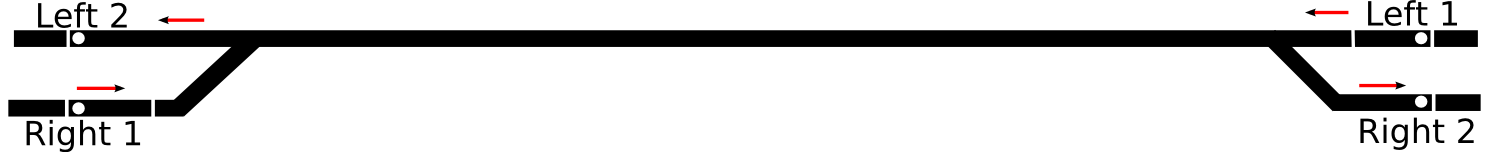
\includegraphics[width=5in]{singletrack-ink1.png}
\caption{Schematic of a bi-direction single track segment}
\label{fig:AutoDispatcher:singletrack-ink1}
\end{centering}
\end{figure}
A schematic track diagram of a bi-direction single track segment is
shown in Figure~\ref{fig:AutoDispatcher:singletrack-ink1}. There are
four sensor locations, shown as white dots and labeled \texttt{Left 1},
\texttt{Left 2}, \texttt{Right 1}, and \texttt{Right 2}.  These sensors
are connected to two MRD2-U, \texttt{Left} and \texttt{Right}. The
sensors are connected to the MRD2-U such that a given MRD2-U's ``sense
1'' is the entry and ``sense 2'' is the exit.  Each MRD2-U device thus
senses a train going in a specific direction through the single track
segment. There is a gap (eg with insulating rail joiners) between both
mainline tracks and the single track segment.  There is an additional
gap about the length of the engine past the entrance sensor.  This short
segment of track is powered via diodes from the rest of the single track
segment. The diodes enforce the correct direction of travel for the
entering train. The single track segment is considered occupied by a train
traveling from right to left if either of the left sensors are active
(the train is entering or leaving) or if the left sensor 1 latch is set
(the train is between sensors).  The  single track segment is
considered occupied by a train traveling from left to right if either
of the right sensors are active (the train is entering or leaving) or
if the right sensor 1 latch is set (the train is between sensors). 
When a train arrives at a sensor 1 position (either \texttt{Left 1} or
\texttt{Right 1}), the computer checks to see if the single track
segment is occupied by a train going in the opposite direction.




%
\cleardoublepage
\bibliography{MRR}
\bibliographystyle{plain}
\cleardoublepage
\printindex
\end{document}



